\begin{proofbox}
	\textbf{\textcolor{CProof}{证明前先问：怎样说明“后者追不上前者”？}}
	看比值最直接：如果$\frac{\text{较慢的}}{\text{较快的}}\to0$，就说明后者与前者相比越来越小。下面只用\textbf{对数运算和高中导数}来说明。

	\medskip
	\textbf{\textcolor{CProof}{第一步：证明对数增长得比正幂慢}}
	对任意$t>0$和$x\ge1$，有一个好用的不等式：
	\[
		\boxed{\ln x\le\frac{x^t-1}{t}}.
	\]
	\textbf{为什么？}令$h(x)=\frac{x^t-1}{t}-\ln x$，则
	\[
		h'(x)=x^{t-1}-\frac1x=\frac{x^t-1}{x}\ge0,
		\qquad h(1)=0.
	\]
	所以$h(x)\ge0$，不等式成立。这一步只用到“\textbf{导数非负，函数不减}”。

	\begin{center}
	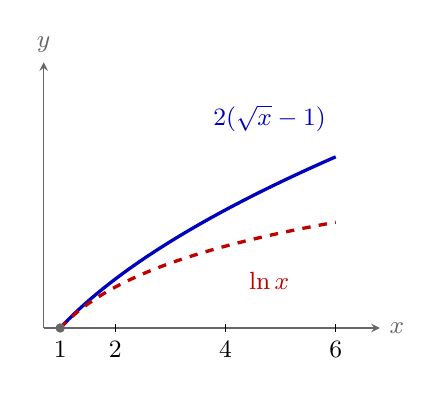
\begin{tikzpicture}[x=0.70cm,y=0.75cm,>=stealth,font=\small]
		\draw[->,gray!80!black] (0.7,0)--(6.8,0) node[right] {$x$};
		\draw[->,gray!80!black] (0.7,0)--(0.7,4.5) node[above] {$y$};
		\foreach \x in {1,2,4,6}{\draw (\x,0.07)--(\x,-0.07) node[below]{\x};}
		\draw[blue!75!black,very thick] plot[domain=1:6,samples=70] (\x,{2*(sqrt(\x)-1)});
		\draw[red!75!black,very thick,dashed] plot[domain=1:6,samples=70] (\x,{ln(\x)});
		\fill[gray!80!black] (1,0) circle (1.7pt);
		\node[anchor=west,blue!75!black] at (3.6,3.55) {$2(\sqrt{x}-1)$};
		\node[anchor=west,red!75!black] at (4.25,.8) {$\ln x$};
	\end{tikzpicture}

	\end{center}
	图上蓝线不低于红线，正是$t=\frac12$时的$\ln x\le2(\sqrt{x}-1)$。图像帮助理解，真正的依据是上面的导数证明。

	\medskip
	现在令$t=\frac\alpha2$。当$x>1$时，因$\ln a>0$，
	\[
		0<\frac{\log_ax}{x^\alpha}
		=\frac{\ln x}{(\ln a)x^\alpha}
		\le\frac{2}{\alpha\ln a}\cdot\frac{1}{x^{\alpha/2}}
		\longrightarrow0.
	\]
	这说明：与$x^\alpha$相比，$\log_ax$占的比例越来越小。因此
	\[
		\boxed{\lim_{x\to+\infty}\frac{x^\alpha}{\log_ax}=+\infty}.
	\]

	\medskip
	\textbf{\textcolor{CProof}{第二步：证明指数最终超过任何正幂}}
	还是用刚才的不等式，不过这次取$t=\frac12$，得到$\ln x\le2(\sqrt x-1)$。
	对$x>1$，把“幂除以指数”取自然对数：
	\[
		\ln\frac{x^\alpha}{a^x}
		=\alpha\ln x-x\ln a
		\le 2\alpha\sqrt x-x\ln a.
	\]
	当$x$足够大（例如$\sqrt x\ge\frac{4\alpha}{\ln a}$）时，
	\[
		2\alpha\sqrt x-x\ln a
		\le-\frac{\ln a}{2}x\longrightarrow-\infty.
	\]
	所以$\ln\frac{x^\alpha}{a^x}\to-\infty$，比值$\frac{x^\alpha}{a^x}\to0$，倒过来便得到
	\[
		\boxed{\lim_{x\to+\infty}\frac{a^x}{x^\alpha}=+\infty}.
	\]
	\textbf{这一步为什么有用？}即使$\alpha=100$、$a=1.01$，只要两个数固定不变，结论仍然成立；可能要等$x$非常大，才看得出指数反超。
\begin{center}
\begin{tikzpicture}[font=\small,>=stealth]
\draw[draw=teal!50!black,fill=green!3,rounded corners=3pt] (0,0) rectangle (13,6.7);
\node at (6.5,6.1) {用比值看领先多少：取 $a=2,\ \alpha=2$};
\begin{scope}[shift={(1.1,1.25)},x=.65cm,y=.34cm]
\draw[gray,->] (1.5,0)--(10.7,0) node[right] {$x$};\draw[gray,->] (2,0)--(2,11.6) node[above] {$r$};
\draw[gray,dashed] (2,1)--(10,1);\node[left] at (2,1) {$1$};
\draw[teal!70!black,very thick,domain=2:10,samples=100] plot(\x,{2^\x/(\x*\x)});
\foreach \x in {2,4,6,8,10}\node[below] at (\x,-.1) {$\x$};
\fill[orange!85!black] (4,1) circle(2.5pt) (8,4) circle(2.5pt) (10,10.24) circle(2.5pt);
\end{scope}
\node[anchor=west,align=left,text width=4.3cm] at (8.3,3.65) {$r=2^x/x^2$\\[10pt]$x=4$：一样大，$r=1$。\\[10pt]$x=8$：指数是幂的 $4$ 倍。\\[10pt]$x=10$：已是 $10.24$ 倍。};
\node at (6.5,.45) {图只展示代表数值；上面的证明说明任意固定 $a>1,\alpha>0$ 的最终趋势。};
\end{tikzpicture}

\end{center}

	\medskip
	\textbf{\textcolor{CProof}{第三步：为什么对数的正数次幂也追不上？}}
	若$\beta>0$，在第一步中改取$t=\frac{\alpha}{2\beta}>0$。当$x>1$时，
	\[
		0<\frac{(\log_ax)^\beta}{x^\alpha}
		\le\left(\frac{1}{t\ln a}\right)^\beta
		\frac{1}{x^{\alpha/2}}\longrightarrow0.
	\]
	因此$x^\alpha/(\log_ax)^\beta\to+\infty$。
\begin{center}
\begin{tikzpicture}[font=\small,>=stealth]
\draw[draw=teal!50!black,fill=green!3,rounded corners=3pt] (0,0) rectangle (13,6.5);
\node at (6.5,5.9) {对数平方也会相对变小：取 $a=2,\ \alpha=1,\ \beta=2$};
\begin{scope}[shift={(1.3,1.5)},x=.045cm,y=2.8cm]
\draw[gray,->] (0,0)--(137,0) node[right] {$x$};\draw[gray,->] (0,0)--(0,1.3) node[above] {$s$};
\draw[gray,dashed] (0,1)--(128,1);\node[left] at (0,1) {$1$};
\draw[teal!70!black,very thick,domain=1:128,samples=200] plot(\x,{(ln(\x)/ln(2))^2/\x});
\foreach \x in {32,64,96,128}\node[below] at (\x,-.03) {$\x$};
\fill[orange!85!black] (8,1.125) circle(2.5pt) (128,.3828125) circle(2.5pt);
\end{scope}
\node[anchor=west,align=left,text width=4.5cm] at (8.1,3.3) {$s=(\log_2x)^2/x$\\[10pt]$x=8$：$s=9/8>1$。\\[10pt]$x=128$：$s=49/128<1$。\\[10pt]开始较大，不妨碍后来占比变小。};
\node at (6.5,.45) {“增长慢”看最终的相对大小，不要求比值从一开始就下降。};
\end{tikzpicture}

\end{center}

	\medskip
	\textbf{\textcolor{CProof}{把证明翻译成大白话}}
	对数相对幂会越来越小；幂相对指数也会越来越小。\textbf{“相差的倍数不断扩大”}才是本结论真正要表达的意思。
\end{proofbox}
